\documentclass{article}
\usepackage[T1]{fontenc}	% for use with pdflatex
\usepackage[utf8]{inputenc} % for use with pdflatex
\usepackage[estonian]{babel}

% paketid
\usepackage{amsmath,amsthm,amsfonts}
\usepackage{graphicx}
\usepackage{listings}
\usepackage{hyperref}
\usepackage{parskip}
\usepackage{abstract}
\usepackage{todonotes}

% eemaldab lühikokkuvõtte pealkirja
\addto{\captionsestonian}{\renewcommand{\abstractname}{}}
\renewcommand{\absnamepos}{empty}

\newtheorem{theorem}{Teoreem}
\newtheorem{corollary}{Järeldus}[theorem]
\newtheorem{lemma}{Lause}
\theoremstyle{definition}
\newtheorem{definition}{Definitsioon}

% matemaatilised ja statistilised operaatorid
\DeclareMathOperator*{\MEAN}{\mathbf{E}}
\DeclareMathOperator*{\VARIANCE}{\mathbf{D}}
\newcommand{\mean}[1]{\MEAN\left[#1\right]}
\newcommand{\variance}[1]{\VARIANCE\left[#1\right]}
\newcommand{\prob}[1]{\Pr\left[#1\right]}

\DeclareMathOperator*{\argmax}{\arg\max}
\DeclareMathOperator*{\argmin}{\arg\min}


% viitesüsteem
\usepackage{biblatex}
\addbibresource{bibliography.bib}

\begin{document}

\title{Spioonid kasarmus}
\author{Reamees \dots}
\date{} % et maketitle kuupäeva ei lisaks

\maketitle
\vspace*{-8mm}

\begin{center}
    {\small Küberväejuhatus \\
    Staabi- ja sidepataljon \\
    Ämari, Eesti}
\end{center}

\begin{abstract}
    \todo[inline]{abstrakt}
    \textbf{Lühikokkuvõte.} \\
    \textbf{Märksõnad:}
\end{abstract}

\section{Sissejuhatus}

\todo[inline]{sissejuhatus}

\section{Taust ja definitsiooonid}

Toome välja mõned definitsioonid koos täiendava taustainfoga, mis töös esinevad.
\todo[inline]{juttu}

\begin{definition}[\cite{juhuslikud-protsessid}]
    \textbf{Juhuslikuks protsessiks} nimetatakse juhuslike suuruste peret $\{ X(t) , t \in T \}$, mille iga liige $X(t)$ on juhuslik suurus tavalises mõistes. Eeldame, et kõik juhuslikud suurused $X(t)$ on määratud ühel ja samal tõenäosusruumil $(\Omega, \mathcal{F}, \Pr)$.
\end{definition}

Parameeter $t$ on sageli reaalarvuline muutuja, mida tõlgendatakse ajana. Mõnikord suhtutakse parameetrisse kui kohta ruumis, mida võib väljendada näiteks vektoriga. Selles töös tähistame parameetriga $t$ aega.

\begin{definition}[\cite{juhuslikud-protsessid}]
    Hulka $T$ nimetatakse juhusliku protsessi \textbf{indekshulgaks}.
\end{definition}

Kui indekshulk $T$ on loenduv nimetatakse protsessi diskreetse ajaga protsessiks. Selles töös mõõdame aega sündmuste toimumiste vahel, seega on mõistlik indekshulka suhtuda kui poolsirgesse $T= [0, \infty]$, siis on tegu pideva ajaga protsessiga.

Matemaatiliste mudelite loomisel päriseluliste olukordade kirjeldamiseks tuleb alati teha lihtsutsavaid eeldusi. Kui üritame olukorda täpselt modelleerida võime arvutustesse ära uppuda. See-eest tehes liiga palju lihtsustusi ei pruugi mudel enam vastata tegelikkusele. Üks sageli tehtud eeldus on, et kindlad juhuslikud suurused on eksponentjaotusega. Eeldus on asjakohane, sest eksponentjaotusega seotud arvutused on lihtsasti järgitavad ning tulemused on sageli head lähendid tegelikkusele. \cite[lk 291]{introduction-to-probability-models}

\begin{definition}[\cite{tõenäosusteooria-algkursus}]
    \label{def:eksponentjaotus}
    Õeldakse, et juhuslik suurus $X$ on \textbf{eksponentjaotusega} parameetriga $\lambda$, $\lambda > 0$ ja tähistatakse $X \sim \mathcal{E}(\lambda)$, kui tema tihedus on
    \begin{equation*}
        f_X(t) = 
        \begin{cases}
            \lambda e^{- \lambda t} ,   &t \geq 0 \\
            0 ,                         &t < 0
        \end{cases}
        \enspace .
    \end{equation*}
\end{definition}

Definitsiooni \ref{def:eksponentjaotus} põhjal võime lihtsasti leida juhusliku suuruse $X \sim \mathcal{E}(\lambda)$ jaotusfunktsiooni

\begin{equation*}
    F_X(t) = \int_{- \infty}^{t} f_X(t) dt = 
    \begin{cases}
        1 - e^{- \lambda t} ,   &t \geq 0 \\
        0 ,                     &t < 0
    \end{cases}
    \enspace .
\end{equation*}

\todo[inline]{esimene lause ja tõestusele järgnev on kordused}
Omadus, mis eksponentjaotust tesitest pidevatest jaotustest eristab on selle 'mälutus'. Kui mingi eseme eluiga on eksponentjaotusega, on kümme tundi (või mingi muu aja) kasutuses olnud ese tõenäosuslikult sama hea kui uus ese tema järelejäänud eluea mõttes \cite[lk 291]{introduction-to-probability-models}. Näiteks on kümme tundi põlenud lambi läbipõlemise tõenäosus viie tunni pärast sama, mis uhiuue lambi läbipõlemise tõenäosus sama aja pärast. Formaalselt võime 'mälutuse' omaduse sõnastada järgneva lausega.

\begin{lemma}
    Olgu $X \sim \mathcal{E}(\lambda)$, iga $t, s \geq 0$ korral $\prob{X \geq t + s \mid X \geq s} = \prob{X \geq t}$.
\end{lemma}

\begin{proof}
    \begin{equation*}
        \prob{X \geq t + s \mid X \geq s} = \frac{\prob{X \geq t + s}}{\prob{X \geq s}} = \frac{e^{- \lambda (t + s)}}{e^{- \lambda s}} = e^{- \lambda t} = \prob{X \geq t} \enspace .
    \end{equation*}
\end{proof}

Lisaks ekponentjaotuse mälutuse omadusele, on võimalik näidata, et see on ainuke pidev jaotus sellise omadusega \cite[lk 296]{introduction-to-probability-models}.

\todo[inline]{üleminek loendavale protsessile}

\begin{definition}[\cite{juhuslikud-protsessid}]
    Juhuslikku protsessi $\{ N(t) , t \geq 0 \}$ nimetatakse \textbf{loendavaks protsessiks}, kui $N(t)$ on mingite sündmuste toimumiste koguarv ajavahemikus $[0, t]$.
\end{definition}

\todo[inline]{ilusam sõnastus}
Üks üldiselt ning selles töös käsitletud oluliseim loendav protsess on Poissoni protsess.

\todo[inline]{definitsioon lühemaks}
\begin{definition}[\cite{juhuslikud-protsessid}]
    Loendavat protsessi $\{ N(t) , t \geq 0 \}$ nimetatakse \textbf{Poissoni protsessiks}, kui
    \begin{enumerate}
        \item $N(0) = 0$, 
        \item iga $t_1 \leq t_2 \leq t_3 \leq t_4$ korral on juhuslikud suurused $N(t_4) - N(t_3)$ ja $N(t_2) - N(t_1)$ sõltumatud, ehk protsessi juurdekasvud lõikumatutes ajavahemikes on sõltumatud,
        \item suvaliste $s, t \geq 0$ korral
        \begin{equation*}
            \prob{N(t + s) - N(s) = n} = \frac{(\lambda t)^n}{n!} e^{- \lambda t} , n = 0, 1, 2, 3, \dots \enspace ,
        \end{equation*}
        teisisõnu on sündmuste arv mistahes lõigul pikkusega $t$ Poissoni jaotusega juhuslik suurus keskväärtusega $\lambda t$.
    \end{enumerate}
\end{definition}

\todo[inline]{ei tea kas see vajalik on}
Kolmandast tingimusest järledub, et $\mean{N(t)} = \mean{N(t)- N(0)} = \lambda t$. Suurust $\lambda$ nimetatakse protsessi \textbf{intensiivsuseks}.

\todo[inline]{kas eemaldada see definitsioon, või lühem tingimus 3 eelmisest}
\begin{definition}[\cite{tõenäosusteooria-algkursus}]
    Õeldakse, et juhuslik suurus $X$ on \textbf{Poissoni jaotusega} parameetriga $\lambda$ ja tähistatakse $X \sim \mathcal{P}(\lambda)$, kui $X$ võimalikud väärtused on $0, 1, 2, 3, \dots$ ning
    \begin{equation*}
        \prob{X = n} = \frac{\lambda^n}{n!} e^{- \lambda} \enspace .
    \end{equation*}
\end{definition}

Tähtis omadus, mis seob omavahel Poissoni protsessi ning eespool välja toodud eksponentjaotuse, on sündmuste toimumiste vahelise aja jaotus. Olgu $\{ N(t) , t \geq 0 \}$ Poissoni protsess intensiivsusega $\lambda$, tähistame sündmuste toimumishetked $S_1 \leq S_2 \leq \dots$ ning ajavehemikud järjestike sündmuste vahel $T_1 = S_1 , T_2 = S_2 - S_1 , T_3 = S_3 - S_2 , \dots$.

\begin{theorem}[{\cite[lk 38]{juhuslikud-protsessid}}]
    \label{trm:tühemikud}
    Tühemikud $T_1 , T_2 , \dots$ on sõltumatud sama jaotusega juhuslikud suurused, $T_i \sim \mathcal{E}(\lambda)$.
\end{theorem}

\todo[inline]{juttu}

\section{Andmed}

Andmepunktid on ajahetked esitatud kellaajaga ISO 8601 formaadis minuti täpsusega. Ajahetke loeme andmepunktiks järgmiste tingimuste kehtivuse korral

\todo[inline]{juttu ja parem definitsioon}

\begin{enumerate}
    \item viimase minuti jooksul ei ole esinenud ühtegi helilist teadaannet spiooni väljasaatmise kohta,
    \item vähemalt üks inimene seltskonnas väljendab pahameelt teda ümbritsevate spioonidega seotud lõhnade kohta.
\end{enumerate}

\todo[inline]{veel jooniseid, algseid/lisatud infoga}

\todo[inline]{järgnev kustuta/tee ümber}
Spioonide esinemissagedust mõjutab luureoperatsiooni korraldaja täis kõht. Kui ressursse on rohkem on võimalik ka rohkem spioone välja saata. Andmpunktid võivad viidata sellele, et peale sööki esinevad spioonid sagedamini. Sellest tulenevalt võib andmetest saada parema ülevaate vaadates spioonide esnemissagedusi söögikordade kaupa, mitte päevade kaupa.

\todo[inline]{vajab ka täpsustusi}
Lisaks spioonide esinemissagedusele tuleb märkida, et pahatahtliku luureoperatsiooni korraldaja saadetud spioonide kohta saab infot vaid siis, kui saadetud spioonid avastatakse. Enamus kirja pandud spioonidest avastati vabal- või reservajal, kui õpperühm paiknes siseruumides ilma suurema tegevuseta.

\todo[inline]{joonis võiks ilusam olla}
\begin{figure}[t]
    \centering
    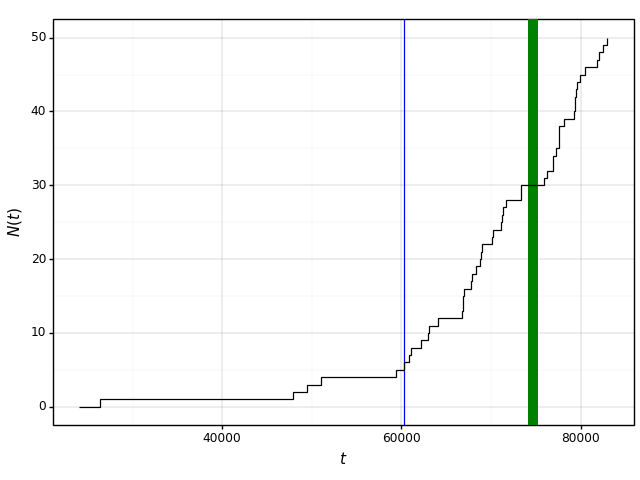
\includegraphics[width=0.8\textwidth]{spioonid_astmejoonis.png}
    \vspace*{-5mm}
    \caption{Spioonide esinemisi loendav protsess alates hommikusest äratusest, sinisega tähistame reservaja algust ning punasega õhtuse rivistuse lõppu.}
    \label{fig:spioonid astmejoonis}
\end{figure}

\todo[inline]{joonise seletus}

\section{Stohhastiline mudel}

\todo[inline]{sissejuhatus}

Tühemike teoreemi \ref{trm:tühemikud} põhjal on võimalik leida hinnang meid huvitava Poissoni protsessi $\{ N(t) , t \geq 0 \}$ intensiivsusele $\lambda$. Selleks tuleb lähendada tühemike jaotuse keskväärtust. Leiame tühemiku $T \sim \mathcal{E}(\lambda)$ keskväärtuse

\todo[inline]{võibolla lihtsalt postuleeri}
\begin{equation*}
    \mean{T} = \int_{- \infty}^{\infty} t f_T(t) dt = \int_{0}^{\infty} t \lambda e^{- \lambda t} dt \enspace ,
\end{equation*}

millest muutujate $u = t$ ja $dv = \lambda e^{- \lambda t} dt$ korral ositi integreerides saame

\todo[inline]{ositi integreerimine}
\begin{equation}
    \label{eq:eksponentjaotus keskväärtus}
    \mean{T} = \dots = \frac{1}{\lambda} \enspace .
\end{equation}

Tulenevalt keskväärtusest \eqref{eq:eksponentjaotus keskväärtus} saame hinnagu intensiivsusele kui leiame valimikeskmise pöördväärtuse

\begin{equation}
    \label{eq:homogeenne intesiivsus hinnang}
    \hat{\lambda} = \left( \frac{1}{n} \sum_{i = 1}^{n} x_i \right)^{-1} \enspace ,
\end{equation}

\todo[inline]{mingile kirjandusele viidates saaks põhjendada, et hinnang on nihketa (näiteks E. M. Tiit rakendusstat) võibolla tasuks ka näidata, et suurima tõepära meetod annab sama tulemuse}
\todo[inline]{kusagil peab formaalselt valimi ja andmepunktid defineerima}
kus $x_i$ on andmepunkt ning $n$ valimi suurus.

\subsection{Mittehomogeenne mudel}

Joonise \ref{fig:spioonid astmejoonis} põhjal on ilmne, et protsess ei ole homogeenne. Seega ei pruugi me valemi \eqref{eq:homogeenne intesiivsus hinnang} põhjal arvutatud intensiivsuse hinnanguga saada tegelikkusele hästi vastavaid tulemusi.
\todo[inline]{sissejuhatus ajalise parameetriga intesiivsusele, ilmselt ka protsessi definitsioon asümptootiliste $o$ hinnagutega}
\todo[inline]{alternatiivina on ainukesed huvipakkuvad ajad joonisel \ref{fig:spioonid astmejoonis} tähistatud, seega saaks uurida üksneid neid piirkondi homogeense protsessina}

\begin{equation*}
    \lambda(t) =
    \begin{cases}
        a , &t < 60 000 \lor 74 500 < t < 75 000 \\
        b , &mujal \\
    \end{cases}
    \enspace .
\end{equation*}

\subsection{Hazard rate}

\todo[inline]{hazard rate, kui see huvitav ei ole võib vahele jätta}

\section{Kokkuvõte}

\todo[inline]{kokkuvõte}

% bibliograafia
\addcontentsline{toc}{section}{Kasutatud allikad}
\printbibliography[title={Kasutatud allikad}]

\end{document}